%!TEX root = ../../report.tex
\section{Content-based Recommender Systems}
\label{sec:content}

\subsection{The functionality of a content-based RS}
The overall reason to implement a Content-based recommender system is basically the same as for other recommender systems; to deliver a list of recommendations that statistically will be seen as valuable to the user. Where it differentiates itself from the others is in the way these recommendations are generated. A content-based recommender system will try to recommend items to the user similar to items that the user has either bought or somehow interacted with in the past. So, in other words, the way the content-based recommender system approaches the recommendation process is by analyzing a set of descriptions of the previously mentioned items which has already been rated or interacted with by the user, and from this information build up a model around the user’s interests. The item preferences from this model will then be compared with those items from the Represented Items repository (see picture). The result returned from the system is a mathematical indication of the relevance these objects or items will represent for the user. As an example, this could help filter search result for webpages. If a resulting webpage has a negative score in comparison to the users interests, it will simply be removed from (or not added to) the list of recommendations.

\subsection{The architecture and modules of the system}
In this section we will describe the different components which substantiates the content-based recommender system by creating the user profile, comparing the user profile with the items contained in the system, and finally by choosing and presenting the recommended items to the user. 
There are three main steps used in the recommendation process, they are described below as follows; content analysis, profile learning, and filtering (see picture).

\begin{figure}[ht!]
\centering
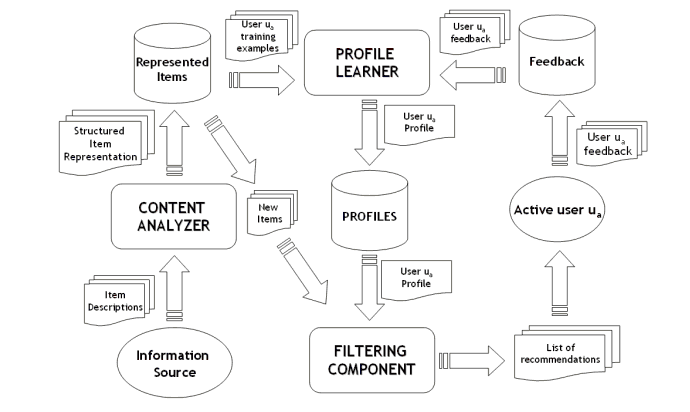
\includegraphics[width=90mm]{Pictures/contentdescription.png}
\caption{source: http://pyevolve.sourceforge.net/wordpress/?p=2497}
\label{contentdescription}
\end{figure}
\todo{Insert reference for illustration to Recommender Systems Handbook}
\begin{itemize}
	\item Content Analyzer: When data has no apparent structure to it, such as text, a processing step which can extract the relevance from the material in a structured way is needed. The main responsibility of the Content Analyzer is to represent data (items, webpages, articles, documents, etc.) in such a way, that it can be used by the next processing steps. This is done by shifting the content representation from its original form to a form usable by the target module (this could for instance be a webpage represented as keyword vectors) via a specific extraction technique.
	\item Profile Learner: This module collect and utilize the relevant information that has been analyzed and altered into a usable format by the content analyzer. In this case, relevant information is data which represents the users preferences. The profile learner aspires to put this information into the right order, and then use this ordered data to create the user profile for the individual user.
	\item Filtering Component: This module uses the profile representation in question and matches this onto the items in the Represented Items Repository. These items will then be further sorted in relation to the users interests and preferences. The result is generated either as a binary yes or no, or as part of a continuous examination of the item, meaning that perhaps there is not enough information on the user available in order to give a correct judgement of the item, so it is instead put on a "waiting list" until further information on the user can be analyzed.
\end{itemize}
These three components work together to recommend items to the user via a series of steps. These steps are illustrated at the picture below. The first step of the process occurs when the Content Analyzer receives a series of item descriptions from an information source. These descriptions are analyzed in order to extract specific features, such as keywords, from the unstructured text, and end up with a structured representation of the items. These items are stored in the repository Represented Items. In order to create and update the Profile for an active user (Ua) for which the recommendations are required, the system collects information regarding the users behavior in relation to certain items. This information is then stored in the repository Feedback.
During the Profile Learner step, the above mentioned information in Feedback is processed together with the represented items in order to predict the relevance of these in relation to the user. A user can likewise create a profile where his or her area of interest are directly provided, thus making the Feedback part of optional relevance.
There are basically two types of relevance feedback, positive and negative. The positive feedback indicates features that the user are interested in, whereas the negative feedback is an indicator of features that have no interest to the user. 
These types of feedback can be recorded via two different feedback techniques, namely implicit and explicit feedback. Explicit feedback refer to when the user actively makes a decision, such as a rating or evaluation, about a specific item. Implicit feedback refers to when the user does not make any active involvement, and is captured by monitoring and analyzing the user's activities and behavior.
The explicit feedback technique is the easiest way for the Recommender System to make recommendations, since it gives a clear and actual indication of the users preferences. When speaking about the explicit kind of feedback, there are three main approaches: like/dislike, rating, and text comments.
The first option works as a binary scale where the user can either choose to like or dislike an item.
The rating option gives the user a larger scale to rate an item on, this could be from 1-10.
The last option presents the user with a set of text comments from other users in order to aide the user in the decision-making whether to buy or not buy a specific item.\\

All of the above mentioned actions will be stored in the Feedback repository in order to help the Profile Learner create a more comprehensive picture of the users preferences. An advantage of the explicit feedback is that it simplifies the interpretation process of the Recommender System for the specific items in question. A disadvantage can be that the user is required to make an active choice, hence incurring a cognitive load on the user. The implicit feedback is centered around actions that do not require direct user involvement on a cognitive level, but more on their actions in relation to the items in question, such as saving, discarding, bookmarking, etc.\\

In order for the Recommender System to create the User Profile for user Ua, the system must first create a training set from the current repository of reference items. The training set is then used by the Profile Learner to match up against user Ua's preferences in order to build a solid foundation for the user profile. Future items in the Items repository will be matched against the user item preferences via the Filtering Component and, if there is a match, these items will be shown as recommendations to the user. \\

This training set of recommendations will need to be updated on a regular basis in order to keep the recommendations as close to the users current preferences as possible. This is of particular importance since a users preferences are most likely to be in a dynamic state of change over time.


\subsection{Keyword-based Vector Space Model}
The mathematical way in which most content-based recommender systems defines the relevance of an item is by the Vector Space Model, which is a spatial representation of text documents. In this model, each of the documents is represented by a vector in a n-dimensional space where n represents the number of terms or keywords from that particular document that matches a, for the system, overall vocabulary. In simple terms, each vector is giving a weight to each keyword to show how big a relevance or association these specific keywords has to the document in question. 
When using VSM to represent the weight of keywords in documents, there are two things that is important: weighting the keyword and measure the similarity or importance of the document in relation to the keyword.
The weighting scheme most commonly used is TD-IDF weighting.

TFIDF stands for Term Frequency / Inverse Document Frequency. TFIDF as a whole is used to generate a profile for a specific object (item, document, etc.). TFIDF is divided into two parts. The first part is Term Frequency which count the number of occurences of a specific term or keyword in the document being analyzed. TF is usually divided by document length, in order to make sure that a book which have the key term in it eight times, is not favored over a short document which contains the same term four times, since a short document with four occurrences might be of a bigger value to the user than an entire book with only eight occurences. 
Inverse Document Frequency then analyzes how many documents contains this term. The formulas for these calculations will be explained further below in this section. 
If a keyword happens to be experienced or noted quite often over a series of analyzations of several objects, then this specific keyword will not be given too much weight, since the system sees it as too common. On the other hand, if a keyword is distinguishable by it occuring infrequently in the objects as a whole, but frequently in specific objects it will most certainly achieve a higher weight and can be beneficial in order to recommend more precise items according to the users preferences.



The object profile are generated by checking the object keywords (can originate from metadata or the object itself (like a document)). \todo{TALK ABOUT USING REGEX TO GO THROUGH TEXT, OR WAIT WITH THAT UNTIL ITU PROJECT IN CHAPTER 3!?!?} These keywords are then given a weight in relation to their significance.
The user profile are generated by the system by checking the keywords for the objects that the user has previously interacted with (bought, viewed, tagged, etc.).
The object profile and the user profile are compared by the system calculating the angle between the item vector and the users �taste� profile vector. The smaller the angle, the more aligned the item are with the user interests. In many recommender systems, instead of the angle, they use the Cosine to the angle. This means, that the closer the value is to one (the values range from -1 to 1), the closer the vectors are aligned.


How the vector which describes an item is computed

In order to understand the concept of the vector weighting we imagine that we have a content space that holds all the keywords that are relevant to the specific situation that we are in. In this space, each keyword represents its own dimension (there are as many dimensions as there are keywords related to the space). Each object occupies a position or a �spot� in our space, which is defined by a vector value.
Each of our users has a �taste� profile which is also indicated by vectors in our space.

There are several ways in which a vector can be computed, in our case we have outlined the three most common ways.
- In some cases a vector will represent a fact (true/false statement) and can be computed simply by using a boolean value. An example of this can be whether a specific keyword is used in a specific document, or whether a specific actor is in a specific movie. The boolean would be used here because it is simply not possible to give this vector a further notion of intensity.
Another way to compute a vector can be by the number of occurrences, which can help give a bigger notion of intensity for the vector.
Our TFIDF implement both of the above mentioned methods, since it can give us a notion of intensity along with a notion of distinctiveness for the individual vector.\newline

Below is shown the formulas for TF-IDF along with an explanation to each.

TF calculates a value for a specific keyword in relation to how many times it occur in the specific document.
%TF
\[
	\text{TF}(t_{k},d_{j}) = \frac{f_{k,j}}{max_{z}f_{z,j}}
\]

The TF-IDF approach add an extra layer to the TF, by further calculating the keywords occurrences in relation to the documents as a whole.
%TF-IDF
\[
	\text{TF-IDF}(t_{k},d_{j}) = \text{TF}(t_{k},d_{j}) * log{\frac{N}{n_{k}}}
\]

Cosine normalization is used to give all the weights in the calculation a value between 0 and 1, and will ensure that the documents are represented by vectors of equal length.
%cosine normalization
\[
	w_{k,j} = \frac{\text{TF-IDF}(t_{k},d_{j})}{\sqrt{\sum_{s=1}^{|T|} \text{TF-IDF}(t_{s}, d_{j})^2}}
\]

The cosine similarity is used to give an indication of the similarity between two vectors, which can then be used to predict whether a user will be interested in a particular item or not. The result is a value between 0 and 1, where the closer we get to one, the bigger the similarity of the items.

%cosine similarity
\[
	sim({d_{i},d_{j}}) = \frac{\sum_{k}w_{ki}*w_{kj}^2}{\sqrt{\sum_{k}w_{ki}^2}*\sqrt{\sum_{k}w_{kj}^2}}
\]


While some of the challenges of recommender systems is to figure out the right weights and factors to use to compute the recommendations for the users, most of the basic recommender system does not handle interdependencies, since it most often are outside the scope of the systems work area.
An example of an interdependency could be from the movie world where a user might like comedies with violence, and historical documentaries, but do not like historical comedies or violent documentaries (or likes Sean Connery in action movies and Owen Wilson in comedies, but not vice versa). Since we can state that the vectors in this case would be comedies, violence, historical, and documentaries, the system in its basicality will have no chance of interpreting the relationship of the users actual preferences, since the system does not have the notion of multiplying different dimensions together. If taking interdependencies into account is a necessity, it is possible to implement this by using a method called LSI/SVD, which stands for Latent Semantic Indexing/Singular Value Decomposition. LSI/SVD identifies associations and patterns between terms and keywords in a text, and adds an extra dimension to the precision with which it is possible to recommend objects to users. We will not go any further into the functionality of LSI/SVD in the context of this report.

\subsection{Advantages and disadvantages}
When looking at recommender systems from a content-based systems point of view there are several advantages over a recommender system in a collaborative-based form.\\

The three main areas of advantage are user independence, transparency, and new items.
The user independence shows itself in that the content-based recommendations are solely based on the active user's own preferences and does not rely on the interaction of others.
The content-based recommendations are transparent in the way that all its recommendations are clearly based on the list of items placed on the user's list of preferences, and consists of no estimated guesses. The advantage of a content-based recommender system in regards to new items that enters the Represented Items repository, is that these items will not need to be rated prior to being recommended to the users. Here, the only dependency is whether the item is similar enough to the individual users preferences.\\

As well as the above mentioned advantages, a content-based Recommender System also has some disadvantages. The three main areas here are limited content analysis, over-specialization, and new user’s.
The limited content analysis revolves around the fact, that content-based Recommender Systems most often are dependant on domain knowledge. An example of this could be for a movie recommendation. Here, the Recommender System would need to know the actors, director, genre, and alike. If the Content Analyzer does not find a suitable amount of information, then it will be virtually impossible for the Recommender System to distinguish between items correlating with the user preferences and items that are of no interest at all.\linebreak
The disadvantage with over-specialization is that the user will never be recommended any items in a positive unexpected manner. What is meant by this is that the user's personal area of preferences might be somewhat wider than the area of the current information held in the User Profile, but since the recommended items for the individual user is based on a match with the items previously rated by the user, there will never be a recommendation deviating from this. This disadvantage is also referred to as The Serendipity Problem.\linebreak
The new user disadvantage can be sort of a predicament for the Recommender System. The issue here is that in order to give the new user a fair recommendation based on user interests and preferences, the user will need to have rated a certain amount of items for the Filtering Component to compare with. When the new user first create his or her account, the recommender system is somewhat forced to either recommend a set of random items or recommend what the average user would be recommended. In most recommender systems the latter is the solution of choice.

